%\documentstyle[epsf,twocolumn]{jarticle}       %LaTeX2e仕様
\documentclass[twocolumn]{jarticle}     %pLaTeX2e仕様(platex.exeの場合)
%\documentclass[twocolumn]{ujarticle}     %pLaTeX2e仕様(uplatex.exeの場合)
%%%%%%%%%%%%%%%%%%%%%%%%%%%%%%%%%%%%%%%%%%%%%%%%%%%%%%%%%%%%%%
%%
%%  基本バージョン
%%
%%%%%%%%%%%%%%%%%%%%%%%%%%%%%%%%%%%%%%%%%%%%%%%%%%%%%%%%%%%%%%%%
\setlength{\topmargin}{-45pt}
%\setlength{\oddsidemargin}{0cm} 
\setlength{\oddsidemargin}{-7.5mm}
%\setlength{\evensidemargin}{0cm} 
\setlength{\textheight}{24.1cm}
%setlength{\textheight}{25cm} 
\setlength{\textwidth}{17.4cm}
%\setlength{\textwidth}{172mm} 
\setlength{\columnsep}{11mm}

\kanjiskip=.07zw plus.5pt minus.5pt


% 【節が変わるごとに (1.1)(1.2) … (2.1)(2.2) と数式番号をつけるとき】
%\makeatletter
%\renewcommand{\theequation}{%
%\thesection.\arabic{equation}} %\@addtoreset{equation}{section}
%\makeatother

%\renewcommand{\arraystretch}{0.95} 行間の設定

%%%%%%%%%%%%%%%%%%%%%%%%%%%%%%%%%%%%%%%%%%%%%%%%%%%%%%%%
\usepackage[dvipdfmx]{graphicx}   %pLaTeX2e仕様(\documentstyle ->\documentclass)\documentclass[dvipdfmx]{graphicx}
\usepackage[dvipdfmx]{color}
\usepackage[subrefformat=parens]{subcaption}
\usepackage{colortbl}
\usepackage{multicol}
%%%%%%%%%%%%%%%%%%%%%%%%%%%%%%%%%%%%%%%%%%%%%%%%%%%%%%%%

\begin{document}

\twocolumn[
\noindent

\hspace{1em}
\today
\hfill
\ \ 細川 岳大

\vspace{2mm}

\hrule

\begin{center}
{\Large \bf 進捗報告}
\end{center}
\hrule
\vspace{3mm}
]

% ‚ここから 文章 Start!

\section{今週やったこと}

Virtual Adversarial Training(:VAT)とFixMatchの実験をした.

\section{実験1(VAT)}
前回のVATのパラメータを調節した.
表\ref{tb:VAT}にパラメータの設定を示す.
\begin{table}[h]
	\centering
	\caption{実験パラメータ\label{tb:VAT}}
	\scalebox{1.0}{
		\begin{tabular}{|c|c|c|} \hline
			model&\multicolumn{2}{|c|}{9層CNN}\\ \hline\hline
			data set&\multicolumn{2}{|c|}{cifar10}\\ \hline
			train data&labeled&4000\\ \cline{2-3}
			&unlabeled&46000\\ \hline
			batch size&labeled&16\\ \cline{2-3}
			&unlabeled&128\\ \hline
			validation data&\multicolumn{2}{|c|}{10000}\\ \hline\hline
			epoch&\multicolumn{2}{|c|}{200}\\ \hline
			optimizer&\multicolumn{2}{|c|}{Adam(lr=0.002)}\\ \hline\hline
			loss&\multicolumn{2}{|c|}{VAT\_loss}\\ \hline
			param&$\alpha$&2.0\\ \cline{2-3}
			&$\epsilon$&40\\ \cline{2-3}
			&Ip&1\\ \cline{2-3}
			&$\xi$&1e-6 \\ \hline
		\end{tabular}
	}
\end{table}

\subsubsection{結果}
図\ref{fig:loss1},\ref{fig:acc1}に結果を示す.
\begin{figure}[h]
	\centering
	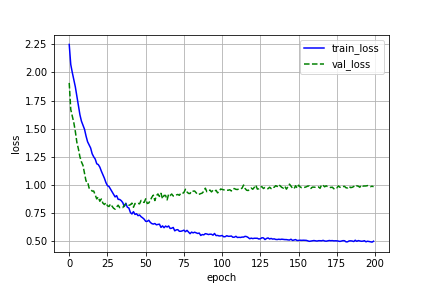
\includegraphics[scale=0.6]{loss_12.png}
	\caption{lossの推移\label{fig:loss1}}
\end{figure}

\begin{figure}[h]
	\centering
	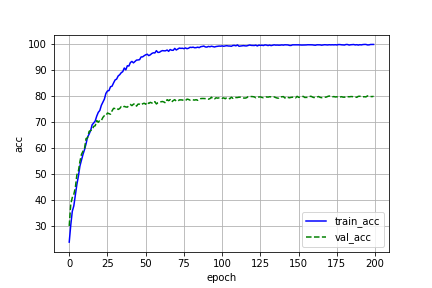
\includegraphics[scale=0.6]{acc_12.png}
	\caption{accuracyの推移\label{fig:acc1}}
\end{figure}

元論文が88\%で,またラベル厚き4000枚のみを用いた実験では70.3\%であったので,
まだパラメータの改善の余地はあるだろうがある程度運用できそうである.


\section{実験2(FixMatch)}
\subsection{概要}
FixMatchとVATの違いについて,
VATではunlabeled\_dataから得られる
lossについて,元画像と微小量のノイズによる変化させた画像とについて予測したものの
kl\_divergenceを付加している.\\
一方で,FixMatchでは弱い変換(translateやflipなど)をした画像で得られた予測を疑似ラベルとし,
強い変換(autocontrastやbrightnessなど)をした画像で得られた予測とのcross\_entropy\_loss
を付加している.\\
この手法をconsistency\_regularizationといい,GANなどにも用いられている.
\subsection{実験設定}
表\ref{tb:Fix}に実験設定を示す.

\begin{table}[h]
	\centering
	\caption{実験パラメータ\label{tb:Fix}}
	\scalebox{1.0}{
		\begin{tabular}{|c|c|c|} \hline
			model&\multicolumn{2}{|c|}{WideResNet28-2}\\ \hline\hline
			data set&\multicolumn{2}{|c|}{cifar10}\\ \hline
			train data&labeled&250\\ \cline{2-3}
			&unlabeled&49750\\ \hline
			batch size&labeled&32\\ \cline{2-3}
			&unlabeled&256\\ \hline
			validation data&\multicolumn{2}{|c|}{10000}\\ \hline\hline
			num\_iterations&\multicolumn{2}{|c|}{$2^{16}$}\\ \hline
			optimizer&\multicolumn{2}{|c|}{SGD(lr=0.1,momntum=0.9)}\\ \hline
			loss&\multicolumn{2}{|c|}{cross\_entropy\_loss}\\ \hline
		\end{tabular}
	}
\end{table}

\subsection{結果}
図\ref{fig:loss2},\ref{fig:loss3},\ref{fig:acc2}に示す.
\begin{figure}[h]
	\centering
	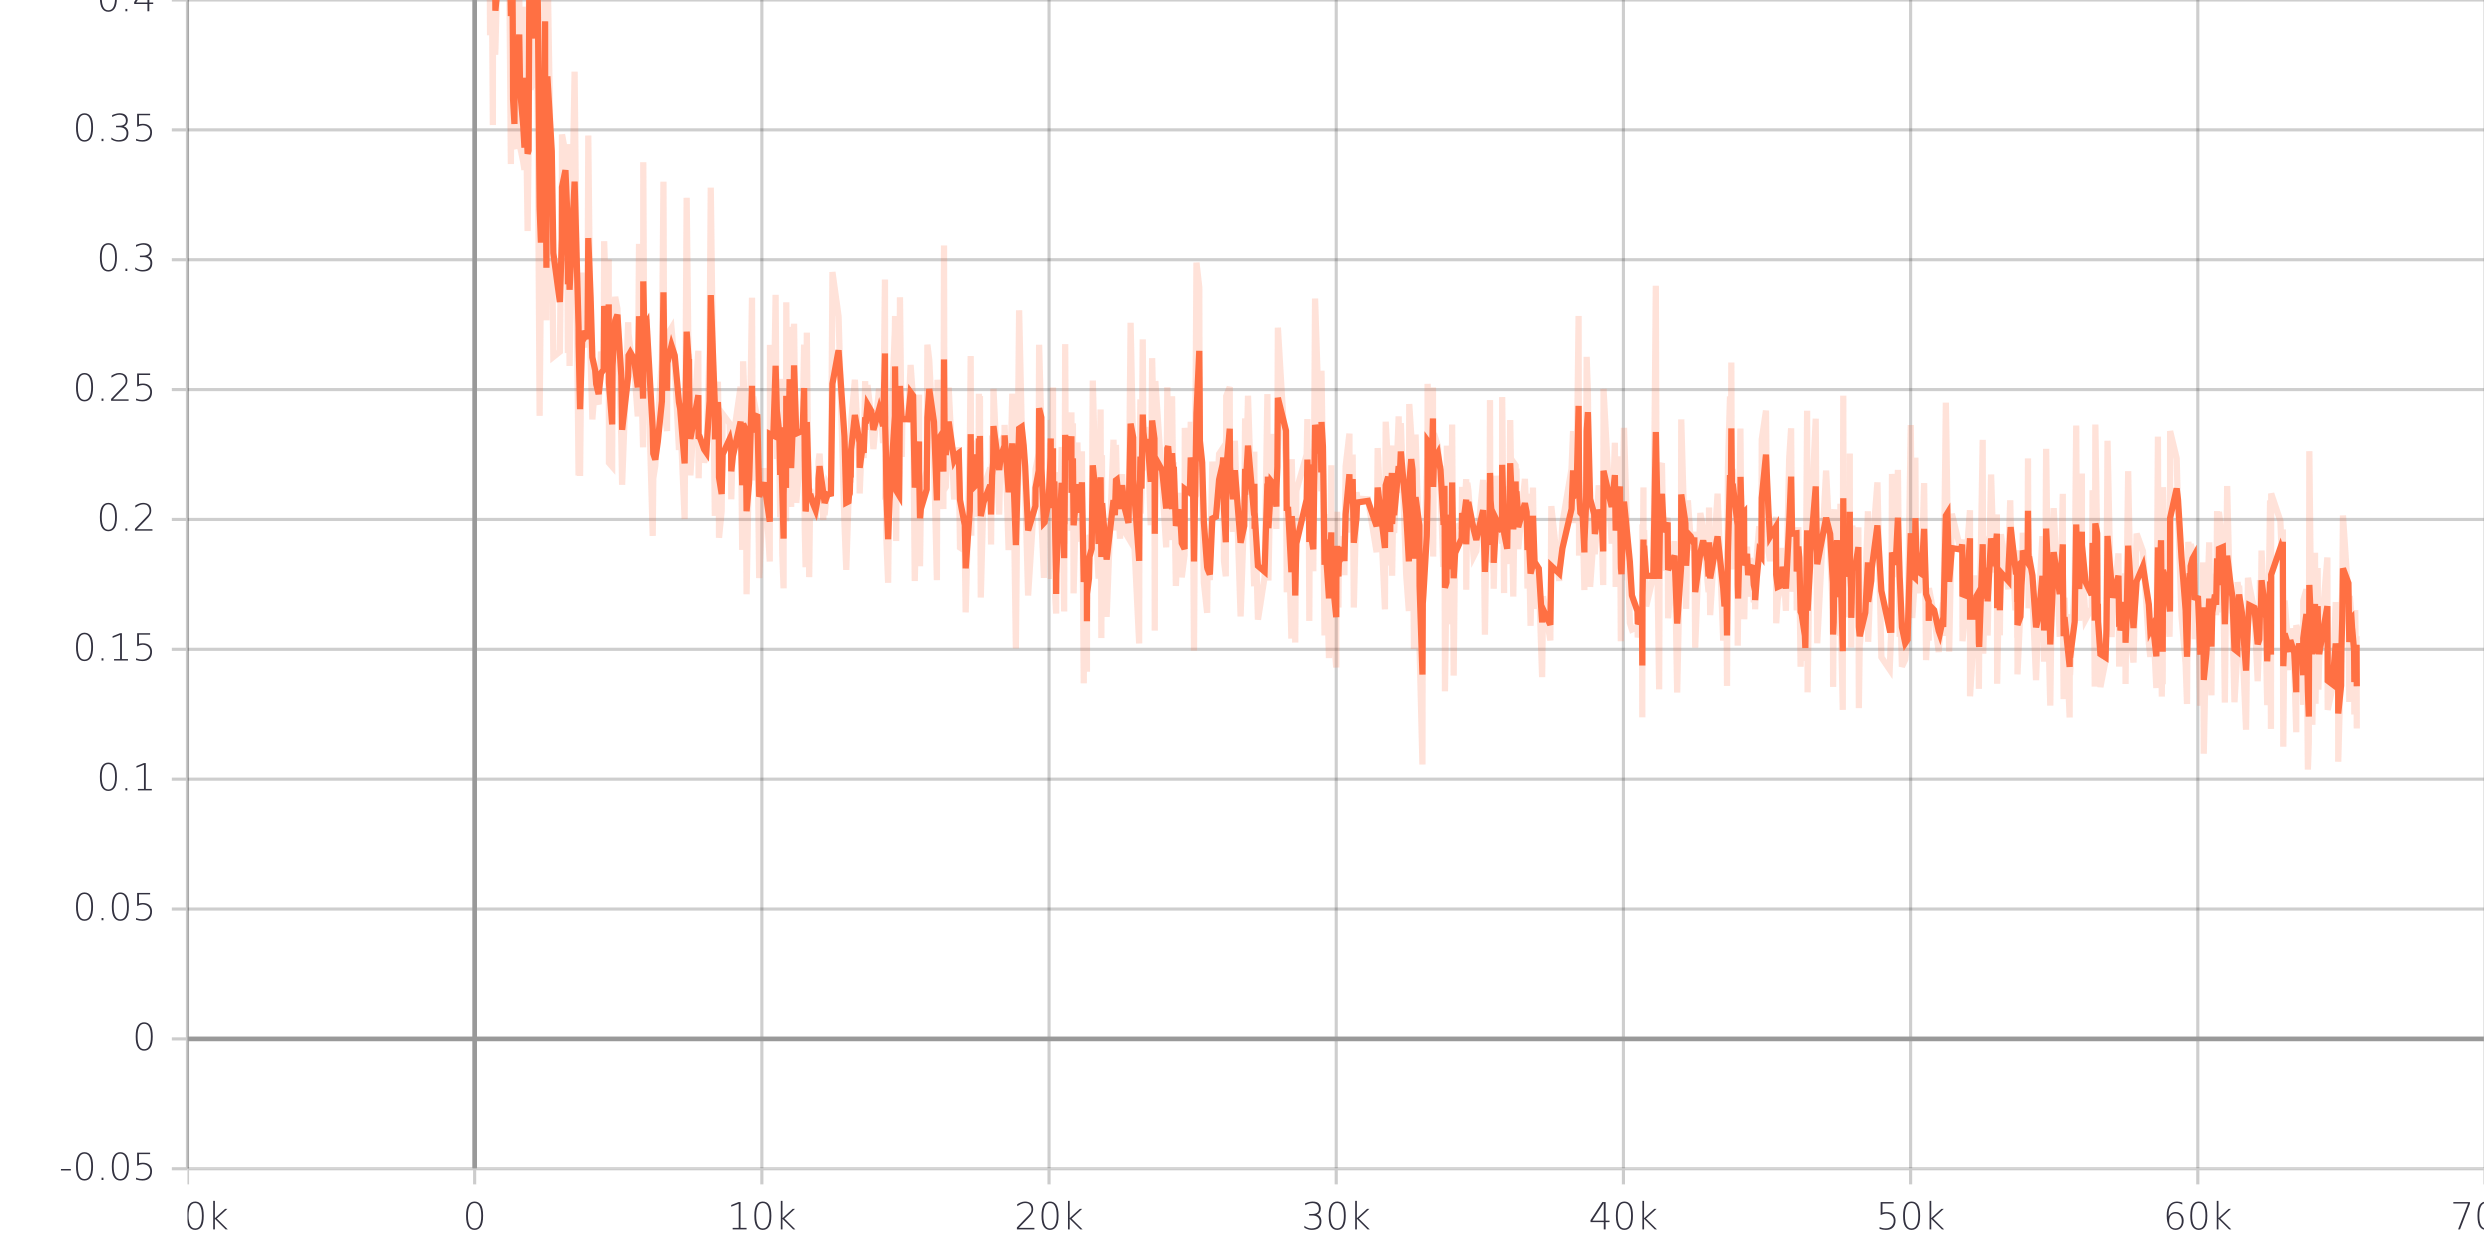
\includegraphics[scale=0.4]{train_total_loss.png}
	\caption{train\_total\_lossの推移\label{fig:loss2}}
\end{figure}
\begin{figure}[h]
	\centering
	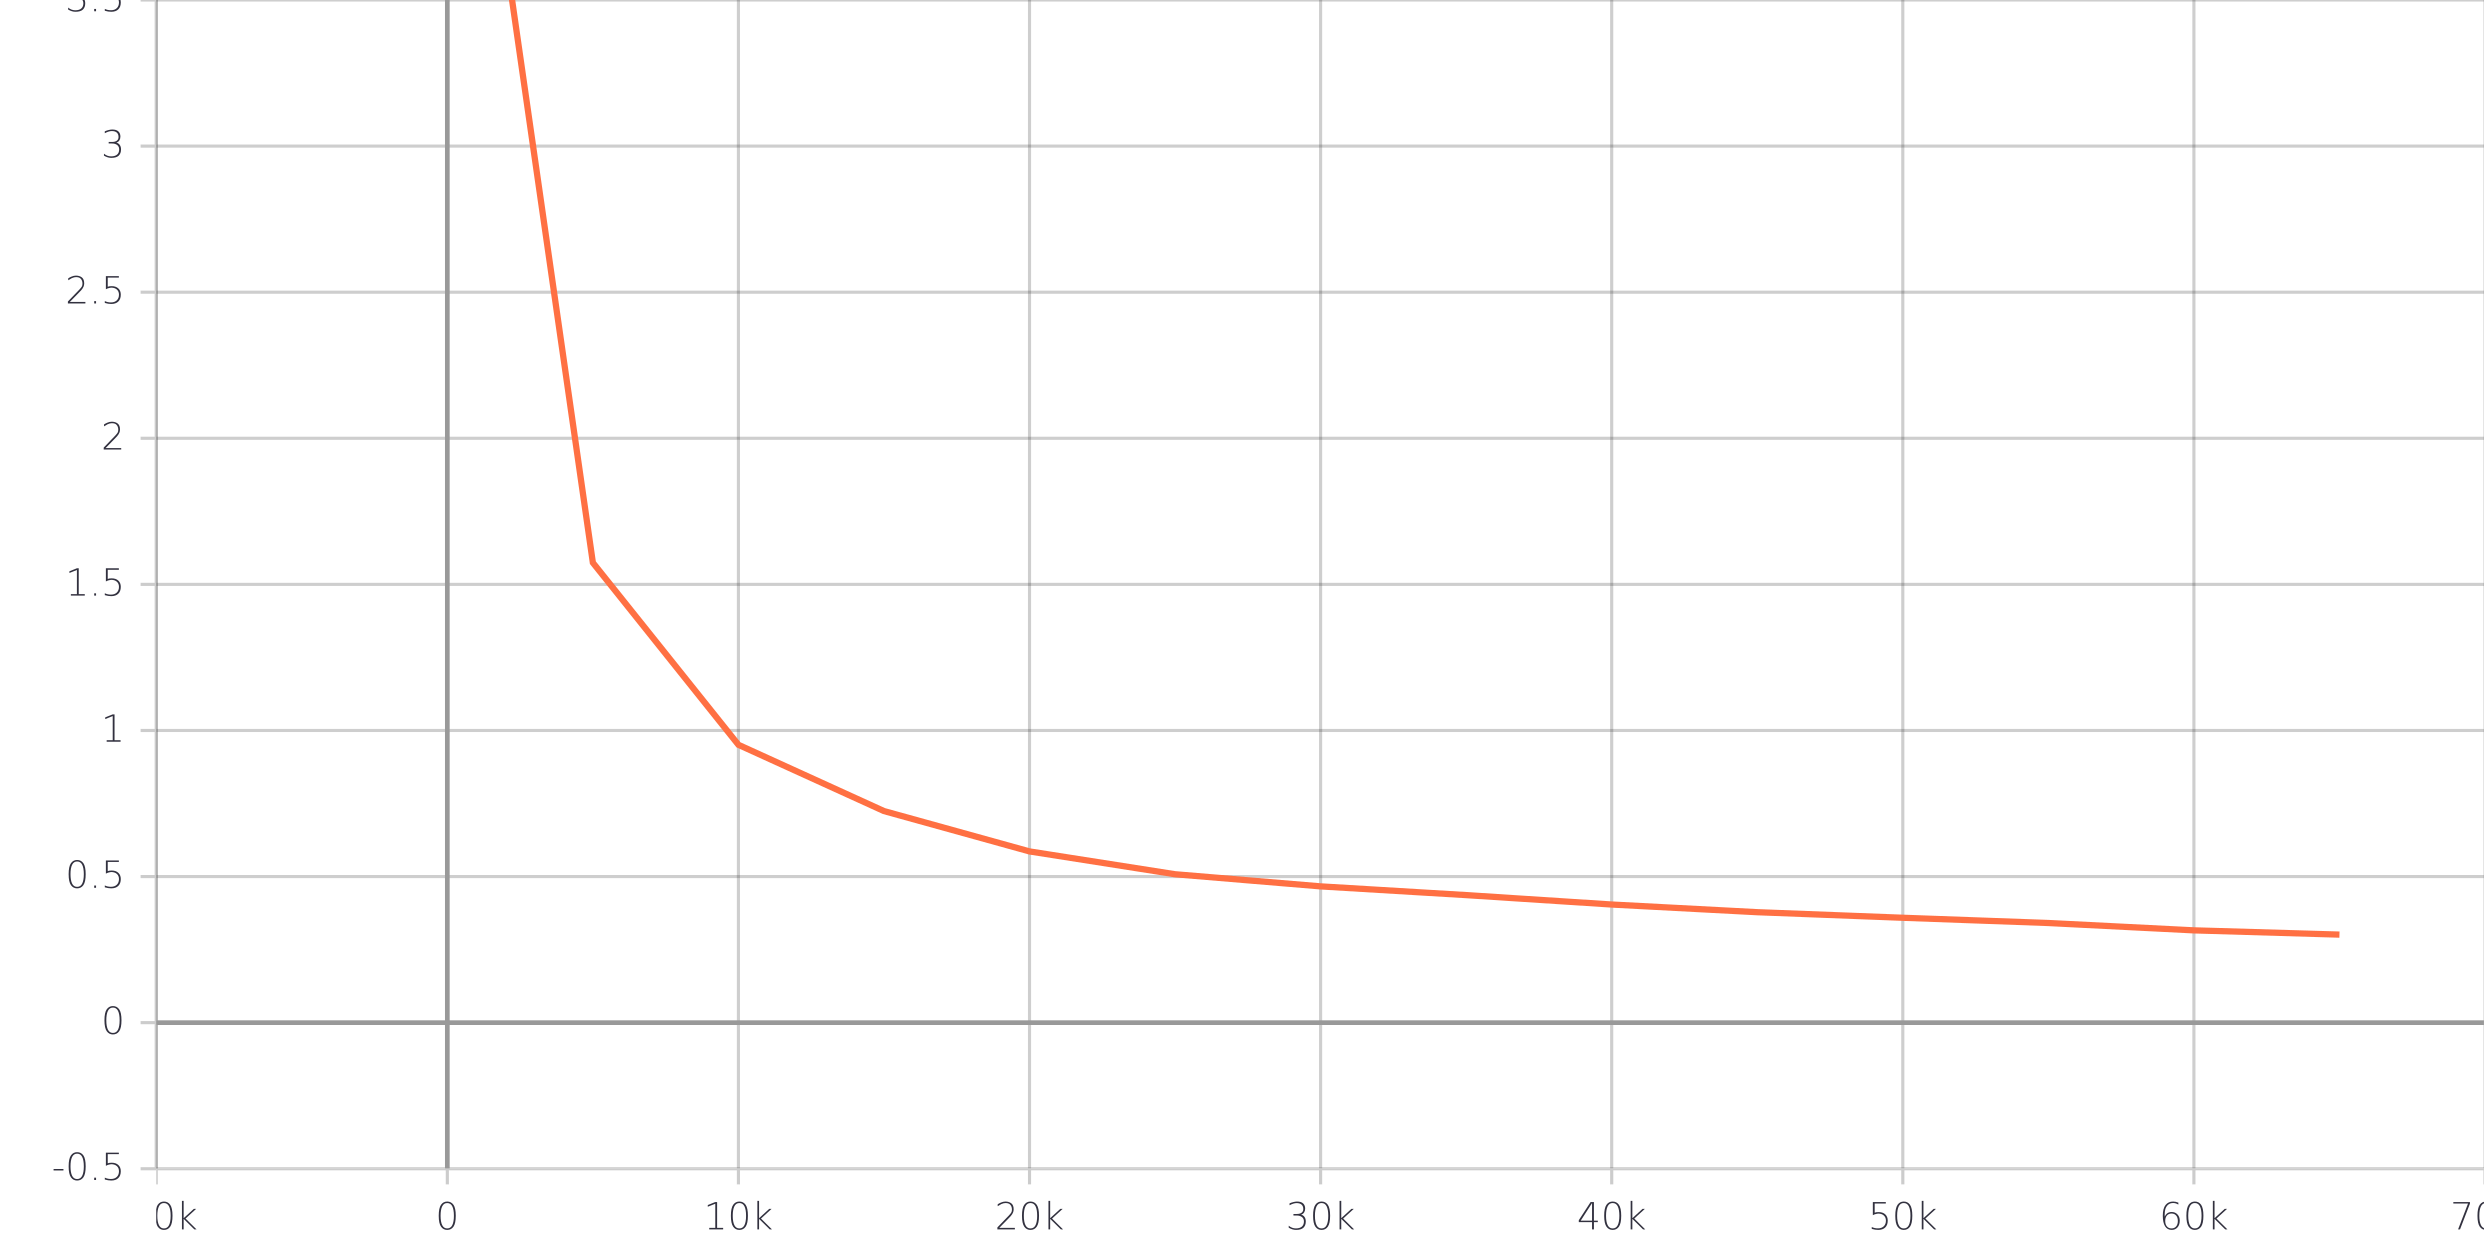
\includegraphics[scale=0.4]{eval_loss.png}
	\caption{validation\_lossの推移\label{fig:loss3}}
\end{figure}

\begin{figure}[h]
	\centering
	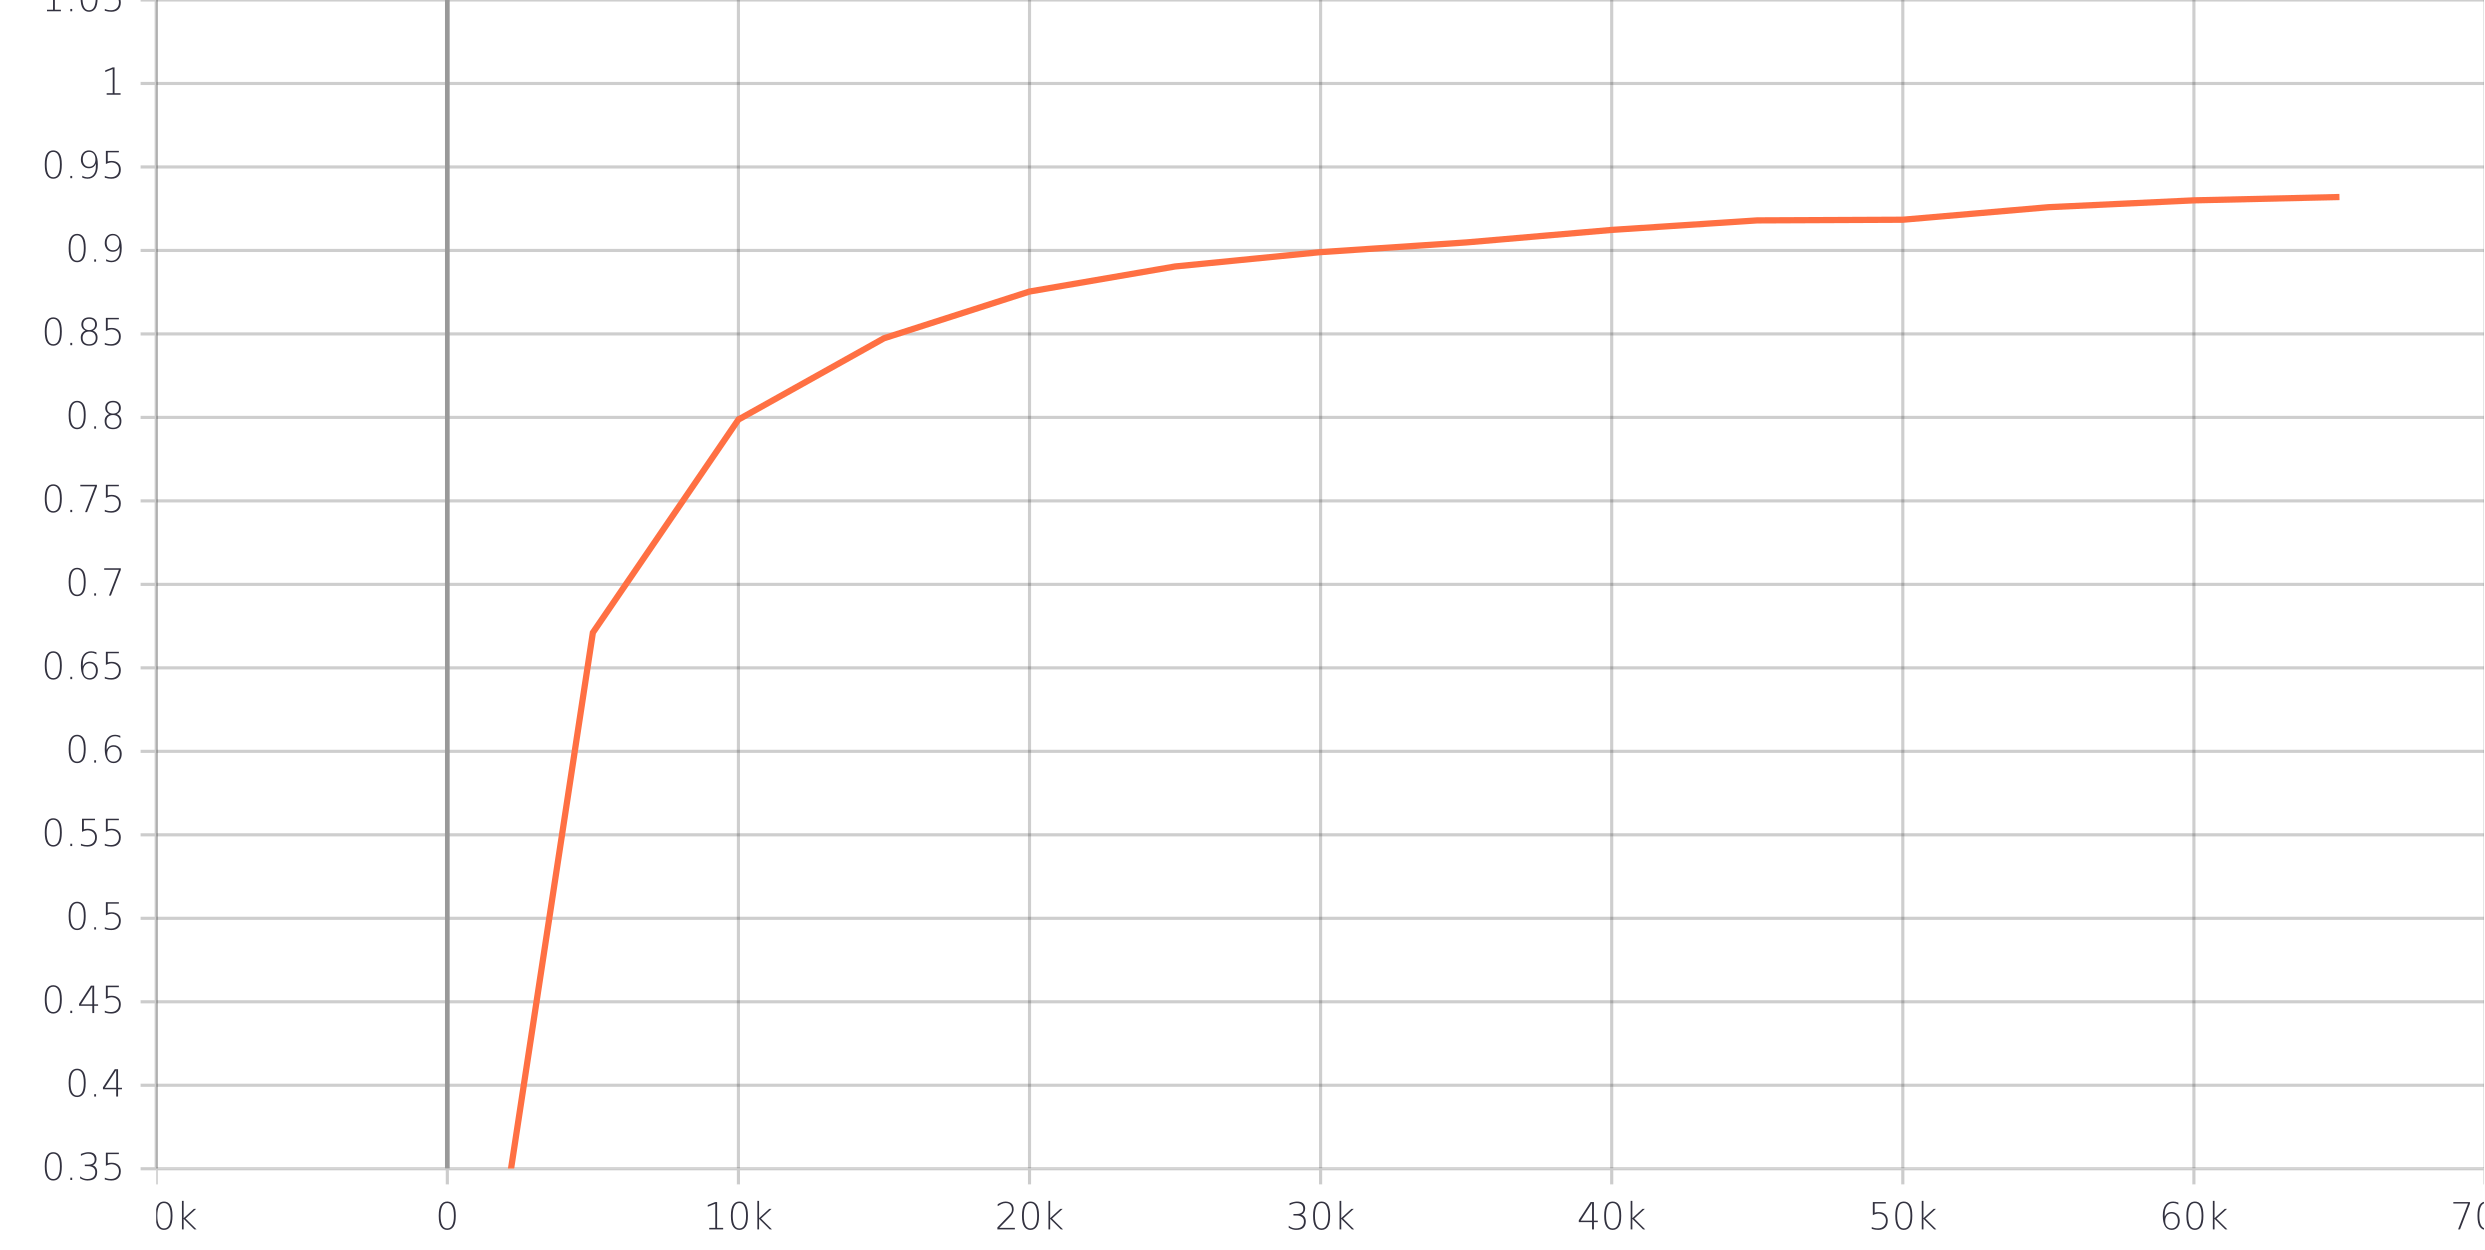
\includegraphics[scale=0.4]{eval_top-1-acc.png}
	\caption{validation\_accの推移\label{fig:acc2}}
\end{figure}
最終的なaccuracyは93.20\%で,元論文が94.93\%であり実験自体はうまく回っているので
次からGAを絡めた実験を行っていく.

\section{考えていること}
GAを用いて,一部のunlabeled\_dataについてlabeled\_dataとして取り扱えるものの選出
をし学習の安定性を図る.\\
validation\_dataとlabeled\_dataの比率を考えた実験を行う.\\
上記二つのアンサンブル学習への転用.

\section{来週の課題}
\begin{itemize}
	\item SSLの実験を進める
\end{itemize}

\end{document}


